\chapter{Implementation} \label{implementation}
Chapter \ref{design} gave an overview about the contents of the prototype application. The requirements as well as the storyline were set. Also, there was a look at how the provided hardware can be used for user interactions in the application. The chapter mentioned the different stakeholders and their tasks and requirements. This chapter will take a look at the application from the developer stakeholder role. It is a documentation of the development process of the VR application. There will be an introduction to the hardware and software tools from a technical point of view. The software architecture will be described as well as problems which occurred during the development and their solutions.

\section{Overview about Unity}
Unity is a multi platform game engine. A game engine holds a bundle of tools which are necessary for game developments such as tools for graphical design, audio and scripting. Game engines support developing games or applications with a lot of 3D and 3D graphics and also supporting developing VR applications.
For the development of this prototype VR application, the game engine Unity and the Occulus Unity SDK is used, which is a support library for Samsung Gear VR and Occulus Go. Unity is the preferred game engine, because it is beginner friendly and free for personal and academic use. Another positive aspect of Unity is the large community from hobby game developers to professional teams. The unity asset store provides many 3D objects, support libraries, textures, audios and other useful tools for game development. This so called assets can be imported into the engine very easily. There is a variety of free assets as well as paid assets. \url{https://sundaysundae.co/unity-vs-unreal/}\\
\begin{figure}[h!]
  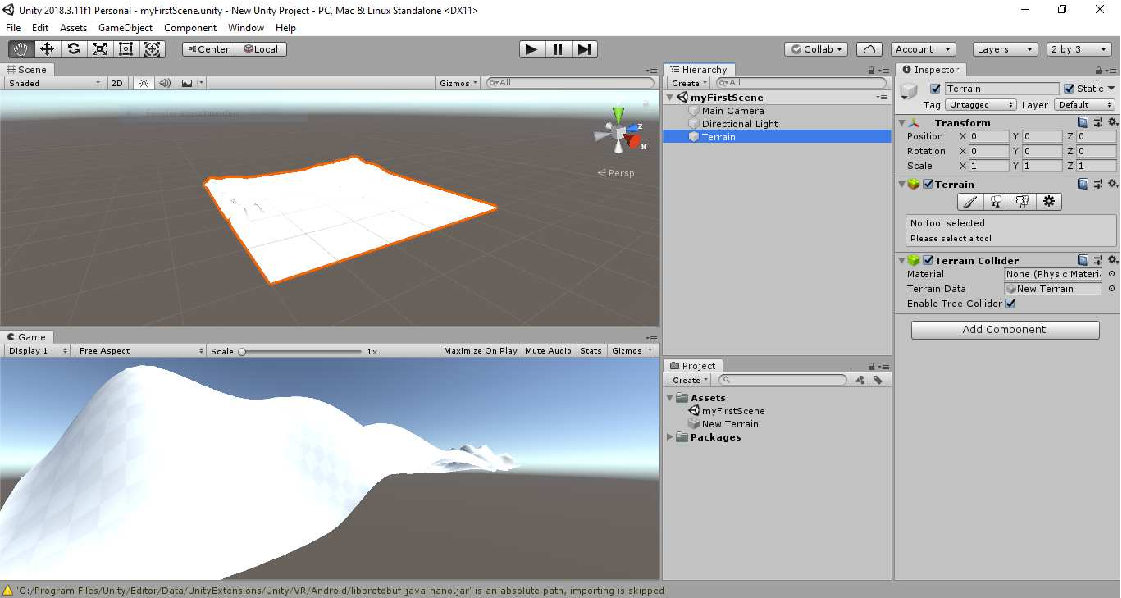
\includegraphics[width=16cm]{kapitel/eps/editor.pdf}
  \centering
  \caption{Screenshot of Unity editor}
  \label{fig:unity-editor}
\end{figure}
The Unity editor, as seen in figure \ref{fig:unity-editor} is the main tool, which is used while creating the prototype. It has a variety of views for designing the environment, modifying and testing the game. \\
In the following, some concepts of Unity will be explained, which are  relevant for the implementation process of the prototype \cite{??}:
\paragraph{Game objects} Game objects in Unity are a very important concept. They can be 3D world objects, lights, cameras and special effects. A game object can also be seen as a container which can contain other game objects. Game objects can be relocated and modified in the unity editor. They can be visible items in the scene or be invisible and work as a trigger area for example.
\paragraph{Components} A component in unity defines a specific property and always belongs to a game object. Every game object can have a variety of components attached. Components can change the appearance and behaviour of a game object in the game. There are several build in components available in unity, but through the scripting API it is possible to create highly customisable components. Unity gives an overview of all components of the selected game object. New components can be attached in the editor.
\paragraph{Prefabs} Prefabs are reusable game objects with components. Once a game object is copied into the prefabs folder in the project, it can be reused between different scenes and even between different projects.
\paragraph{Materials and shaders} Materials can be seen as the skin of game objects. Materials define how the surface of objects look like. The material is a component which can be modified in the Unity editor. Which properties can be edited depends on which shader is selected for the material. Shaders are scripts which define the rendering of the material through algorithms. The shader defines which input parameters can be modified in the material component.

\subsection{Scripting in Unity}
Unity provides a variety of predefined components, which can be attached to game objects, such as a Rigidbody for physical behaviour or an Audio source for playing music. However, for customizing the behaviour of a game object, it is possible to create components and attach a script to it. A script can either be written in C\# or a  modified JavaScript by Unity. For this prototype application, C\# is chosen, because it is the wider used programming language within the Unity community. Every component is a class and inheritates from the MonoBehaviour class. Through the scripting API all existing game objects within the game and their components can be accessed and modified, it is possible to create new game objects, react to events, load new scenes and control the game flow. The MonoBehaviour class contains several methods which can be overwritten to execute code after various lifecycle events. The update method for example is called every frame update of the game object. It can be used  to get continues updated values from the game object for example. The start method is called once before the gameplay starts. This method is mostly used for initialization of other game objects or components.\\
In general, all rules, best practices and design patterns which are common in the .NET environment can be used within Unity as well. Unity uses some special concept of dependency injection, which is very important and will be explained shortly because it is often used in the prototype application: Every object variable which has public access in a class will be visible in the component in the inspector view. It is now possible to inject a reference to that variable by drag and drop a game object or a component to the variable in the inspector view. There is no need to initialize the variable in the code. Public variables of a primitive type can  be directly modified through the inspector view.
\subsection{Unity and Samsung Gear VR support} \label{gearvrsupport}
\todo{describe registering device}
In Unity, VR support can simply be enabled by ticking a box in the player settings. However, to make a game which is compatible with the Samsung Gear VR, more work than that has to be done. First of all, the Occulus support library has to be imported. It can be downloaded from the Unity asset store. This library is shortly introduced in chapter \ref{sdksupport} and contains a variety of components and prefabs. For this prototype the OVRCharacterController prefab from the SDK is used. It contains all necessary scripts and objects for the communication between Unity and the VR hardware. The OVRCharacterController is a first person controller which can be used in the VR environment. It controls the camera from a first person perspective. With the use of this prefab it is also easy to set up the Samsung Gear VR handheld controller support. The prefab contains a script called OVRInput which can register connected controllers and input events. However, the OVRCharacterController prefab is missing a handheld controller representation within the game. The user needs this kind of representation in order to see the movements of their hand while playing the game. Occulus provides a handheld controller game object. This object simply has to be attached to the OVRCharacterController prefab. Once the controller object is attached, the movements of the user's hand get automatically mapped to the virtual controller in the game. To realize selecting and object manipulation with this handheld controller, more adaptions in the code have to be done. How this is solved is described in chapter \ref{inputmethods}.

\section{Implementation of the smart city scene}
According to the storyboard from chapter \ref{storyboard}, the smart city scene is the first scene of the game and the entry point for the different labs, which represent the IT job roles. This section describes the implementation of this scene, including the scene design, the gameplay and the deployment to the HMD. It also describes   solving of challenges which occurred during the implementation, such as the dialogue system and supporting of different input methods.
\subsection{Scene Design}
Before starting to program the game logic, the outlook of the scene has to be designed. This is an important step in the implementation because the look of the environment defines a first impression and is a factor when it comes to immersion. The more realistic the environment is designed, the more present users feel in the virtual world.\\
Skyboxes are a concept in unity to design the background of the game. They contain of a picture wrapped around the scene to give an impression of a wider environment. 
For the prototype, an image with an urban environment is chosen. The image is a 360 photography of a place in a city surrounded by skyscrapers (TODO image). This image gets attached to the skybox component of the main camera. The image is used in all scenes, the world scene as well as the different laboratory scenes, to state out that the user has not left the city. \\
The smart city environment is an urban environment which should look like a South-East-Asian city. The environment should also encourage free exploration. This means that there should be a high level of details and the game objects of the scenes should be of a high quality. To focus the work on the gameplay and on the same time provide a high quality environmental design, a city scene from the Unity asset store is used TODO ref. This scene is adapted in the size and  
\subsection{Implementation of the dialogue system}
The application contains several conversations with the virtual assistant, as seen in chapter \ref{design}. The dialogues between the virtual assistant and the user take place in various places in the game and after different events. The implementation of the dialogue component contains setting the input texts, animating the text appearance during the dialogue, controlling user input and displaying the right dialogue texts at the right time. Especially the last task is a challenge, looking at the fact that the game is organized by unity in a stateless game loop. The dialogue component is implemented as a reusable component. It should be possible to add new sentences or change the appearance of the sentences without significant expense.\\
The dialogue component is a combination of the dialogue script and the dialogue panel, a game object which contains the text and the user input buttons (see figure TODO). The dialogue script is attached to an empty game object named DialogManager. From there, references to the dialogue panel are set. The sentences, which should be displayed by the dialogue system are represented as a string field in the dialogue script. Every entry of a field is the text which should be displayed on the panel. When the user clicks the continue button, the next entry from the string field is displayed. This variable has a public accessory. Therefore the content of the dialogue can be changed by any class at any time. \\
The dialogue script has a public method called StartTyping which invokes displaying of the sentences in the string field with a typewriting animation. It also handles the continue button click by the user. Once every sentence is displayed, the dialogue panel disappears automatically. In the scene controller class, it is only necessary to set the content of the sentences and to invoke the StartTyping method. \\
To display questions and react to answers of the users, it is possible to customize the buttons appearing on the dialogue panel. Every button click invokes a callback, which is an interface method. This interface can be implemented individually by the controller classes. The appearance of the dialogue panel with the right sentences at the right time can also be managed in the controller classes. This is done by implementing a state machine pattern. The DialogManager class holds a reference of a stateMachine variable which is also an interface. The reference is set inside the controller classes. A state machine is an object which implements the IStateMachine interface. The method NextState() performs a step through the state machine. The variable current returns the current state, the state machine is at the moment. Every state describes an event or a position in the game. Because the DialogManager is a reusable component, it should not know in which state the game is currently. The task of the DialogManager class is only to display all referred sentences when the method is invoked. After all sentences are displayed, the NextState() method is called, to let the controller classes know, that the displaying of the dialog is finished. 
\begin{figure}[h!]
  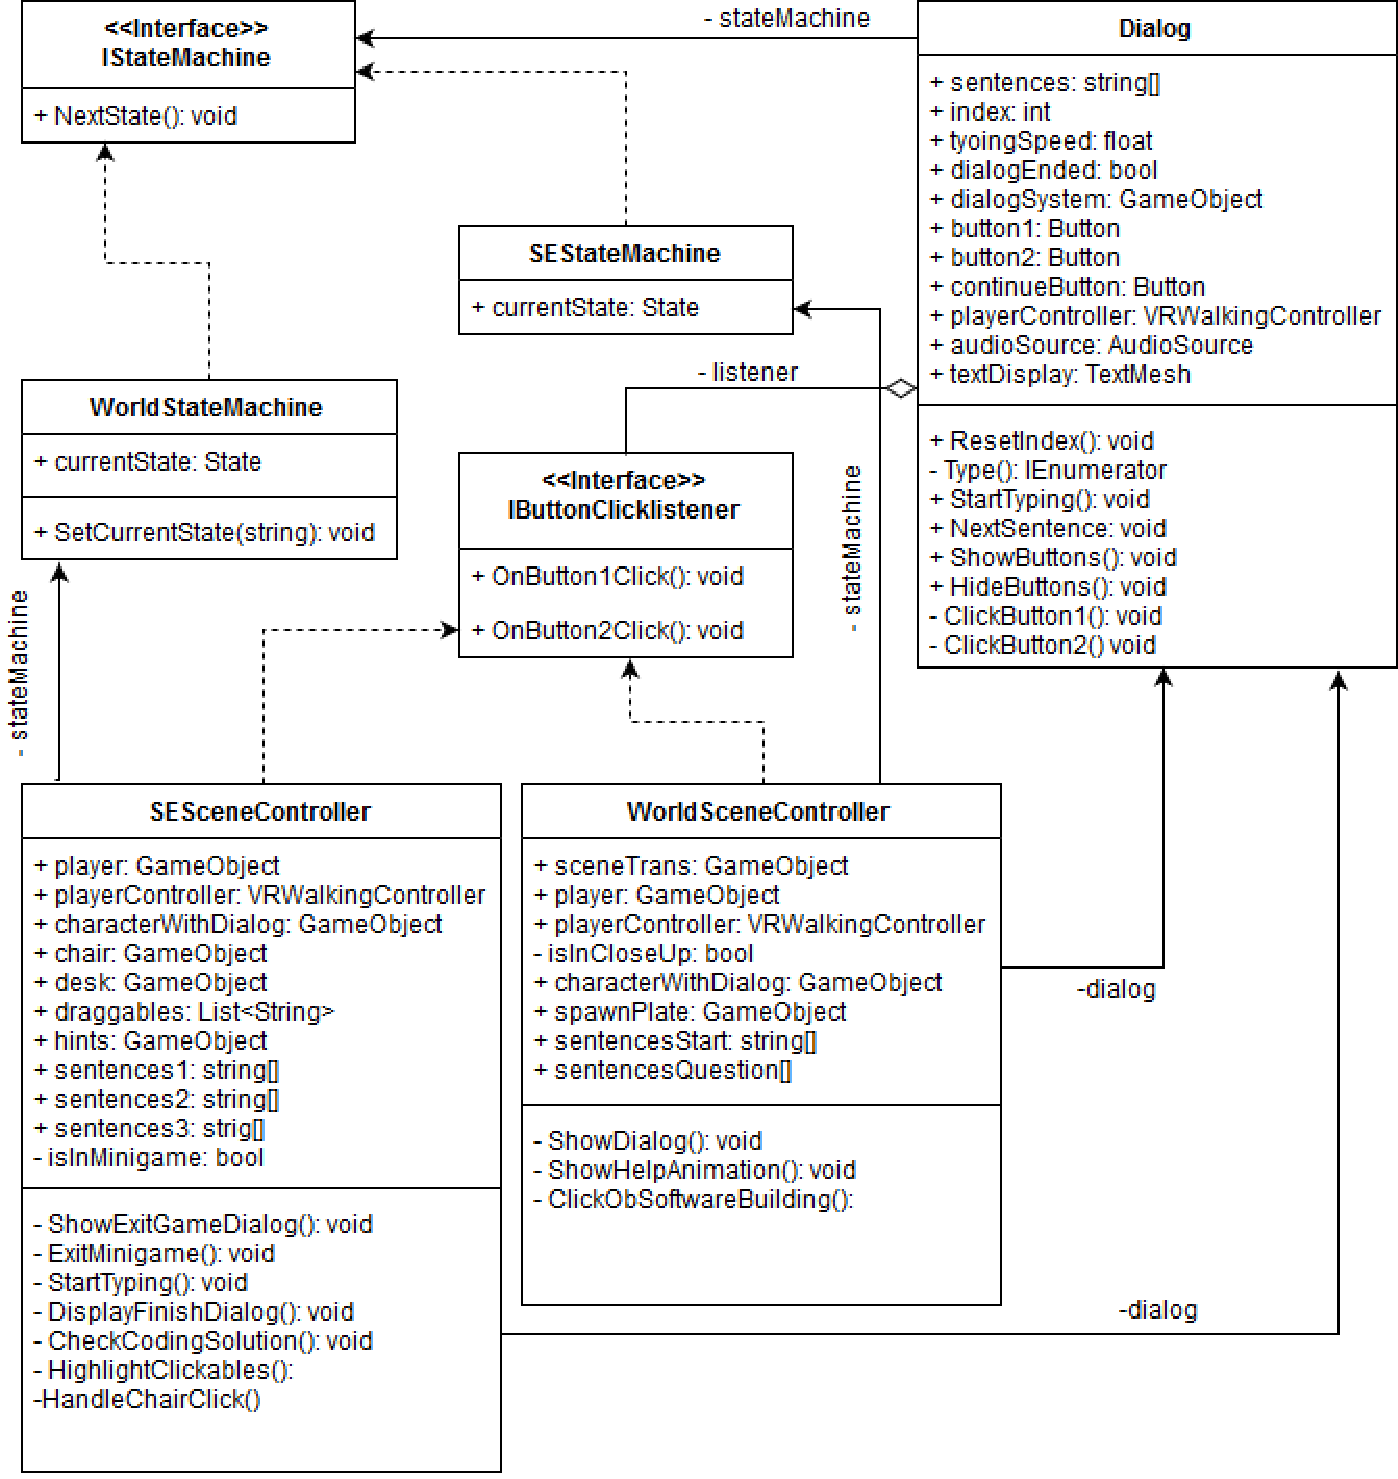
\includegraphics[width=13cm]{kapitel/eps/uml-dialog.pdf}
  \centering
  \caption{UML class diagram for the dialogue component}
  \label{fig:uml-universalinput}
\end{figure}

\subsection{Deploying to VR headset}
\subsection{Support of different input methods}
\label{inputmethods}
Deploying the application to the VR headset takes a few minutes every time. During the development, a continuous testing is necessary. If the testing would always be done on the VR device, it would be too time consuming. Therefore the game is only deployed on the VR headset when some VR specific functions need to be tested. In other cases the game is tested on the desktop. \\
The problem of this procedure is, that the input methods of both target platform differ: For the VR headset, the handeld controller is used, while on the desktop PC mouse and keyboard are the primary input methods. Therefore a solution has to be found, how to make the game playable on both platforms without changing the code when switching the target platforms.

The Samsung Gear VR provides support for user input in different ways. On the right side of the HMD is a touchpad attached. Common gestures like taping and swiping can be performed on the touchpad. The HMD transfers the input commands directly into the VR application. In the implementation of this prototype, the touchpad is not used as an input method. Instead, the Samsung Gear VR handheld controller is used. Nevertheless, the HMD touchpad should be seen as a fallback solution, in case there is no handheld controller available. Adding a support for the HMD touchpad input method is therefore a feature which should be added in the future.\\
The Samsung Gear VR handheld controller can either be used with the left or right hand. This controller is connected to the phone via bluetooth. The controller offers more possibilities for user input than the touchpad at the HMD. Figure \ref{fig:controller} displays the input buttons of the controller in more detail.
A very important feature of the handheld controller is also that the controller has sensors to detect its rotation. With this functionality it is possible to point at objects in the game to select them.\\
\begin{figure}[h!]
  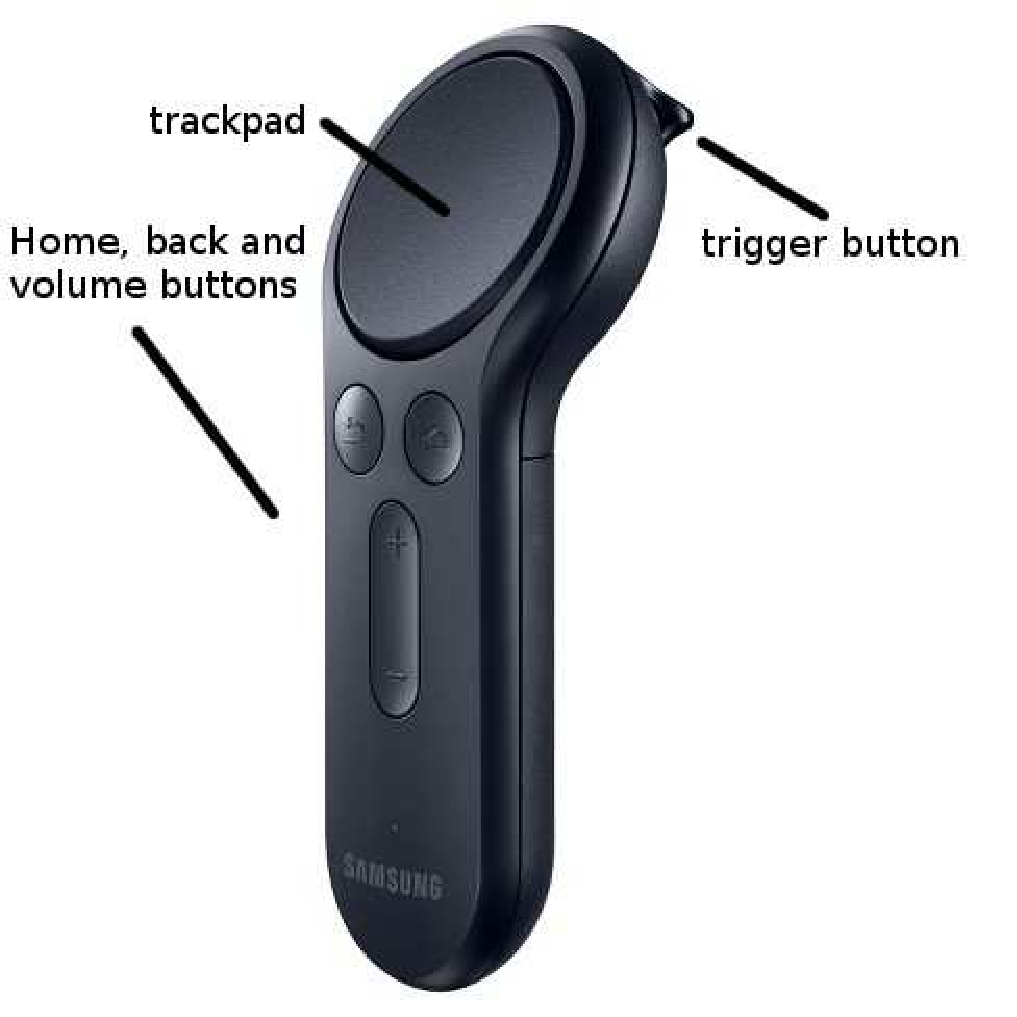
\includegraphics[width=8cm]{kapitel/eps/samsung-controller.pdf}
  \centering
  \caption{Handheld controller with button description. Edited from \cite{Samsung.2019b}}
  \label{fig:controller}
\end{figure}
When switching from the desktop platform to the mobile VR target platform with the handheld controller, following input methods need to be implemented in a different way:
\begin{itemize}
\item Looking around
\item Relocating
\item Selection of objects
\end{itemize}
Looking around in the game is done by a component named MouseLook in the desktop target platform version of the game. This component is a script from the unity standard assets, which is a free utilities library available in the asset store. It manages looking around in a first person view in the direction of the mouse position. When switching the target platform to mobile VR, no mouse position is available, therefore the script does not work. Instead of the MouseLook script, the OVRPlayerController, which was described in chapter \ref{gearvrsupport} is attached to the first person controller. It manages looking around in the direction of the head movement instead of the mouse movement.\\
Relocating on the desktop target platform is done with the WASD keys of the keyboard, an input method used in many computer games. The movement is also implemented by a script from the unity standard assets. However, in a virtual environment it is not possible to use the keyboard. Instead, the relocation is done by pressing the trigger button to move forward with a constant speed. The direction of moving is set by the direction in which the user is currently looking. The implementation of this relocating is very straightforward: TODO insert code.\\
Selection of objects is done with the ray-casting method in both target platforms. How ray-casting in unity works, is seen in example \ref{raycastcode}. The ray is created from the mouse position, which is always the center of the screen. The if condition checks whether the ray hit a game object and returns this object inside the \texttt{hit} variable.
\begin{lstlisting} 
RaycastHit hit;
        Ray ray = camera.ScreenPointToRay(Input.mousePosition);
        
        if (Physics.Raycast(ray, out hit)) {
            Transform objectHit = hit.transform;
        }
\end{lstlisting}
\label{raycastcode}
\captionof{lstlisting}{simple ray-casting }
First of all a ray is created from a fixed starting point. If the ray hit an object, this object is stored as a Hit in the variable hit. The difference of ray-casting on the desktop and the VR version is that the ray comes from the center of the main camera on the desktop version, whereas in the VR version the ray is initialized from the controller model in the game. In order to make the game work on the Samsung Gear VR, the initialization of the ray has to be changed to the example in listing \ref{raycastcode-new}
\begin{lstlisting} 
RaycastHit hit;
        if (Physics.Raycast(controller.transform.position,
         controller.transform.forward, out hit))
        {
            return hit.collider.gameObject;
        }
\end{lstlisting}
\label{raycastcode-new}
\captionof{lstlisting}{Ray initialized from the controller representation in the game}

The method \texttt{Physics.Raycast} creates the ray from the controller's position instead of the center screen this time. The method checks for objects hit by the ray at the same time.
When changing every ray creation which is done in the game's code to the above showed solution, the game is working on the mobile VR platform but it is not working on the desktop target platform or in the unity editor gameplay mode anymore. In order to use ray-casting on every target platform without changing the code every time, an additional class has to be added. This class is able to detect, which is the current target platform and also if the game is running in the editor gameplay mode. The class creates the ray from either the main camera or the current connected controller depending on the current target platform. It is also able to detect, if a controller is connected and if the controller is set as left or right hand used. In the UML-diagram in figure \ref{fig:uml-universalinput}, the UniversalInput class fulfills the above explained functionalities. The UML-diagram shown below only shows the method and fields relevant for the problem case of this chapter. Subclasses which are used by the UniversalInput class are not displayed in the diagram. The controller classes of the different game scenes use the methods of the UniversalInput class to get the selected object from the ray. It is now possible to play the application with the Samsung Gear VR and use the controller to point at selectable objects. At the same time, the game can be played on a desktop with selecting objects through the main camera focus.
\begin{figure}[h!]
  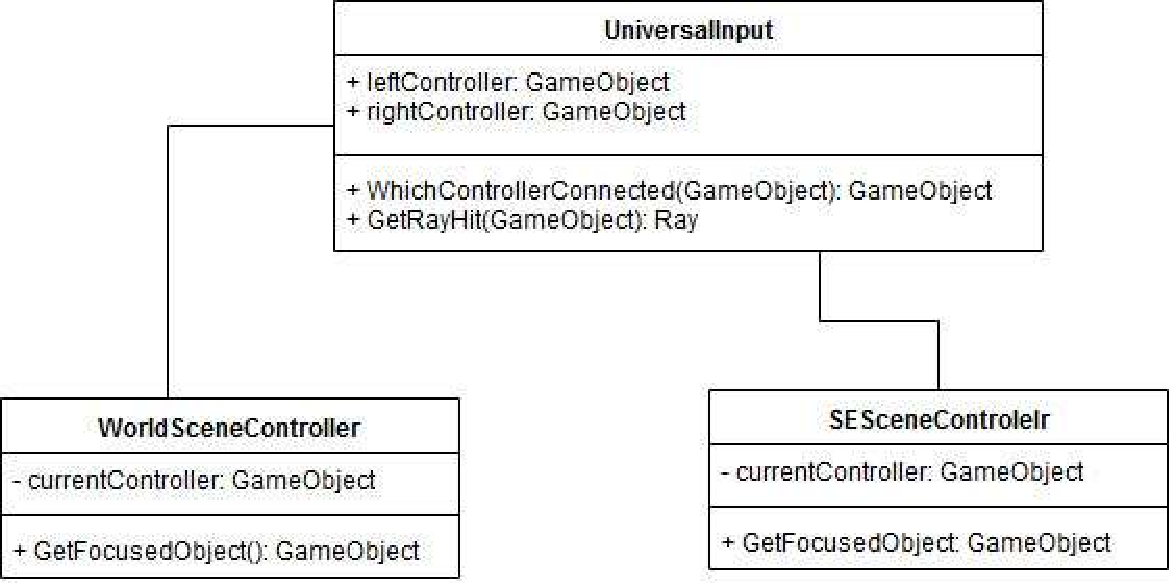
\includegraphics[width=13cm]{kapitel/eps/uml-input.pdf}
  \centering
  \caption{UML class diagram for managing different target platforms}
  \label{fig:uml-universalinput}
\end{figure}
\section{Implementation of the software engineer scene}
\subsection{Coding minigame}
\subsection{User guidance}
\todo{Describe how highlight hover and hint over hand is displayed}

\subsection{Software engineer scene design}
\section{VR specific problems}
--> TODO describe the multi platform feature of unity in more detail.
In the beginning of the implementation, the HMD was not available yet. Therefore, the initial gameplay programming had to be done without the use of VR. Luckily, unity is a multi engine platform, so the development could be done for a desktop pc as a target build. The scene design and the basic gameplay mechanics were done independently from the target platform. \\
However, although the application is able to run on desktop as well as on a mobile device in combination with the Gear VR, some mechanics and the user input concepts differ in each platform. This section describes, what problems occured when switching the target platform to a mobile VR target. It also explains, how the problems were solved. The objective of this section is to make the application runnable and playable on the desktop target platform as well as on the mobile VR target platform without the need to change the code. This is an important requirement, because during the development, a quick testing in the editor gameplay mode is necessary. 

